\chapter{Transmission by layer of last scattering}
\label{ch:lastlayer}

\section{The question}

A particle that reaches the detector at the angle $\twotheta$ had a last scattering in some layer $k$. From there it crossed several layers on its way out,
each one attenuating it. The function \code{transmission_by_last_layer} (module \code{transmission_by_layer.py}) gives one vector for each layer $k$,
\begin{equation}
  T_k(\twotheta)=\Big\langle \exp\!\Big(-\sum_i\mu_iL_i(\twotheta)\Big)\Big\rangle_{\text{last scattering in layer }k},
\end{equation}
where $L_i$ is the path in layer $i$ from the scattering point to the exit of the sample towards the detector. The sum includes \emph{all} the layers crossed,
not only layer $k$.

\section{How ``last scattering'' is defined}

The particles are followed one by one, as in Chapter~\ref{ch:scattering}. At \emph{every scattering event} the question asked is: ``if this were the last
scattering and the particle went to the detector, how much would it be attenuated?'' This is computed with the exact direction of the detector, for
all the angles at once, which gives smooth curves. Each event is classified by the layer where it takes place and by its order:
\begin{description}
  \item[single] the first scattering of the particle;
  \item[multiple] the second or later scattering;
  \item[total] both together.
\end{description}
The result contains the pure attenuation. The probability of being scattered towards the detector (for instance $1/4\pi$ if the scattering is isotropic)
is a common factor that is not included, as in Chapter~\ref{ch:transmission}; the number of scattering events in each layer is given to weight the layers.

\section{Calling the function}

\begin{lstlisting}
res = transmission_by_last_layer(sample, beam_width, beam_height, H=None, V=None,
                                 n_particles=50000, angles_deg=None, phi_deg=0.0,
                                 deflection_sampler=None, max_orders=200, rng=None)
\end{lstlisting}
\begin{center}\small
\begin{tabular}{@{}>{\raggedright\arraybackslash}p{5.6cm}p{9cm}@{}}
  \toprule \textbf{Result} & \textbf{Content} \\ \midrule
  \code{res.angles_deg} & the angles $\twotheta$ (default 0 to 180, step 1) \\
  \code{res.layer_names} & names of the layers \\
  \code{res.transmission[k]} & vector versus angle: last scattering in layer $k$, all orders \\
  \code{res.transmission_single[k]}, \code{res.transmission_multiple[k]} & the same for first scatterings only, and for second and later ones \\
  \code{res.events(kind)[k]} & number of scattering events in layer $k$; \code{kind} is \code{"single"}, \code{"multiple"} or \code{"total"} \\
  \code{res.events(kind)[k] / res.n_incident} & events in layer $k$ per incident particle (weight of the layer) \\
  \code{res.mean_transmission(kind)} & transmission averaged over all the layers, weighted by the events \\ \bottomrule
\end{tabular}
\end{center}
A layer without scattering events (for example a gap with $\mu=0$) gets NaN. The layers are numbered in the order of the sample (for the cylinder, from the
axis outwards). The plot is made with \code{plot_transmission_by_layer(res, kind="all")}, which draws three panels (total, single, multiple); the
legend gives the events per incident particle in each layer.

\pyexample{ex06_by_layer}

\section{Results}

\begin{figure}[ht]
  \centering
  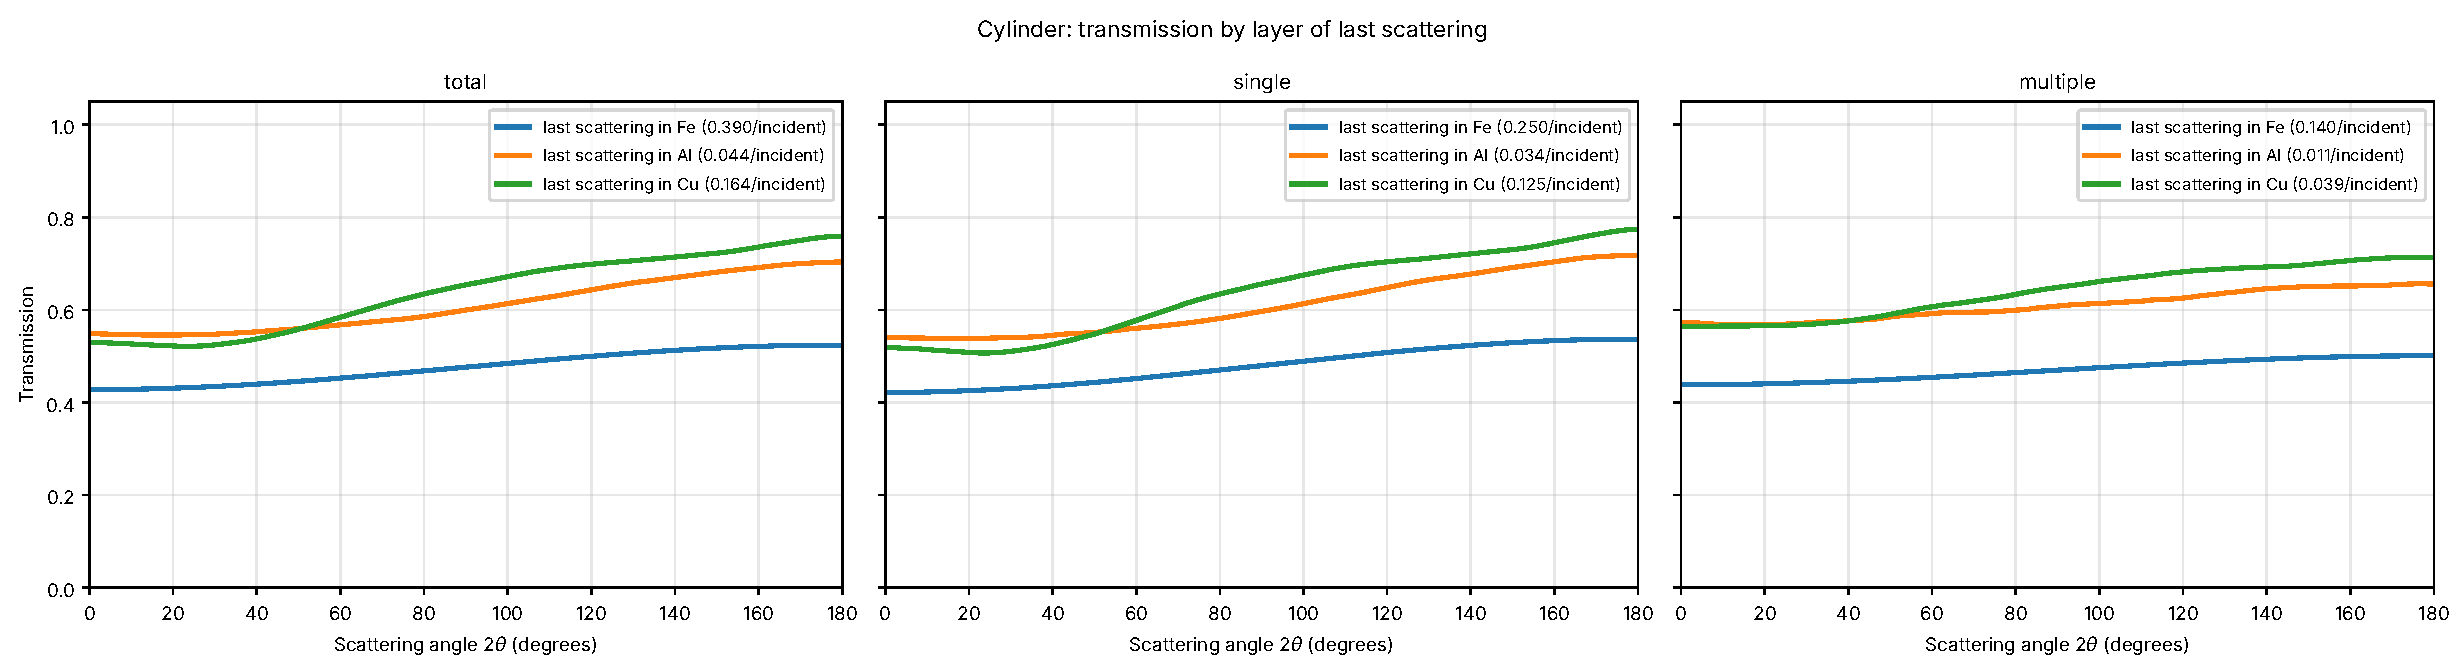
\includegraphics[width=\textwidth]{fig_bylayer_cylinder}
  \caption{Cylinder: transmission versus $\twotheta$ for each layer of last scattering (total, single and multiple scattering). The number in the
  legend is the number of scattering events in that layer per incident particle.}
  \label{fig:blcyl}
\end{figure}

For the cylinder (Figure~\ref{fig:blcyl}), particles whose last scattering was in the inner Fe core have the lowest transmission, since they have to cross the most
material to leave; those scattered in the outer Cu shell are less attenuated, especially towards backward angles. Most of the scattering events take place in the Fe core.

\begin{figure}[ht]
  \centering
  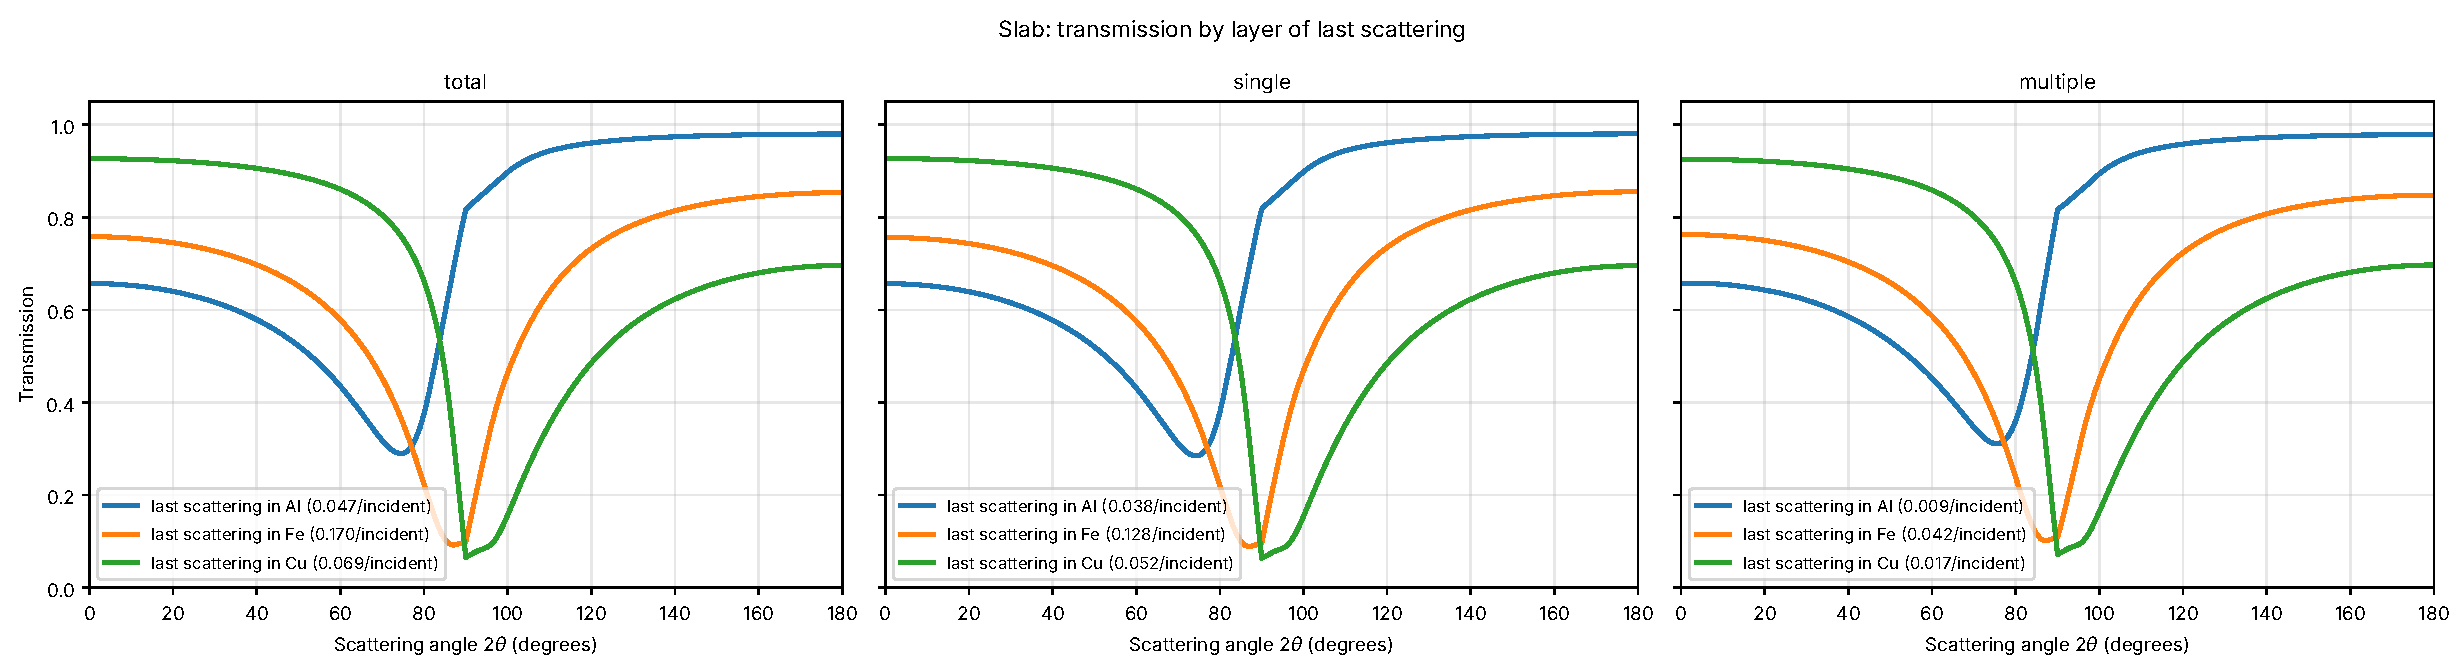
\includegraphics[width=\textwidth]{fig_bylayer_slab}
  \caption{Slab perpendicular to the beam: the same quantity. The steps near $90^\circ$ are real: just below $90^\circ$ a particle scattered in the
  first layer must cross all the others to leave through the back face, whereas just above $90^\circ$ it leaves backwards through the first layer only.}
  \label{fig:blslab}
\end{figure}

\section{Relation with the other functions}

If all the layers have \code{scatter_fraction}\,=\,1, the \emph{single} result averaged over the layers with \code{res.mean_transmission("single")}
is identical (to rounding) to the transmission of Chapter~\ref{ch:transmission}. The \emph{multiple} part is consistent, within the statistical
errors, with the particle-by-particle counts of Chapter~\ref{ch:scattering} (Chapter~\ref{ch:validation}).
